\documentclass{beamer}
\usepackage[utf8]{inputenc}
\usepackage{amsmath}
\usetheme{CambridgeUS}
\usecolortheme{beaver}

\title[Generating logo images with GANs]{Generating logo images with \\ Generative Adversarial Networks}

\author[Todorov, Kanev, Vellev]{
 Hristo Todorov
 \and
 Hristo Kanev
 \\
 \and
 Scientific advisors: Dr. Stoyan Vellev
}
\begin{document}
\frame{\titlepage}

\begin{frame}
\frametitle{Introduction}
\begin{itemize}
\item What are we trying to achieve?
\item How are we trying to achieve it?
\item What is the main question we want to answer?
\end{itemize}
\end{frame}

\begin{frame}
\frametitle{Dataset}
\begin{itemize}
\item Large Logo Dataset (LLD)
\item Composed of over 600 000 high-quality diverse images
\item Can be used freely for academic purposes
\begin{figure}[ht]
    \centering
    \includegraphics[scale=0.35]{lld.png}
    \caption{Sample images from the dataset}
    \label{fig:dataset}
\end{figure}
\end{itemize}
\end{frame}

\begin{frame}
\frametitle{Generative Adversarial Networks}
\begin{figure}[ht]
    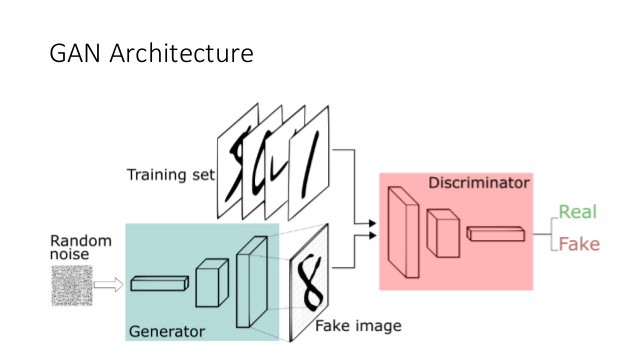
\includegraphics[scale=0.27]{gan_architecture.jpg}
    \caption{Architecture of a GAN}
    \label{fig:gan}
\end{figure}

\end{frame}

\begin{frame}
\frametitle{Training a Generative Adversarial Network}
\begin{itemize}
\item Trained via backpropagation - no need for any Markov chains
\item Really unstable to train
\item The loss (cost) function heavily affects the training process
\end{itemize}
\begin{block}{Binary cross-entropy}
\begin{equation}
\min_G \max_D V(D, G) = \mathbb{E}_{x\sim p_{data}(x)}[\log D(x)]
    + \mathbb{E}_{z\sim p_z(z)}[\log(1 - D(G(z)))]
\end{equation}
\end{block}
\begin{block}{Least Squares Loss}
\begin{equation}
\min_D{V_{LSGAN}} = \frac{1}{2}\mathbb{E}_{x\sim p_{data}(x)}[(D(x) - 1)^2] + \frac{1}{2}\mathbb{E}_{z\sim p_{z}(z)}[(D(G(z))^2]
\end{equation}

\begin{equation}
\min_G{V_{LSGAN}} = \frac{1}{2}\mathbb{E}_{z\sim p_{z}(z)}[(D(G(z))^2]
\end{equation}
\end{block}
\end{frame}

\begin{frame}
\frametitle{Wasserstein Generative Adversarial Network}
\begin{itemize}
\item Minimal changes to the architecture of the discriminator
\item Harder to train
\item No sign of vanishing gradients and mode collapse
\end{itemize}
\begin{figure}[ht]
    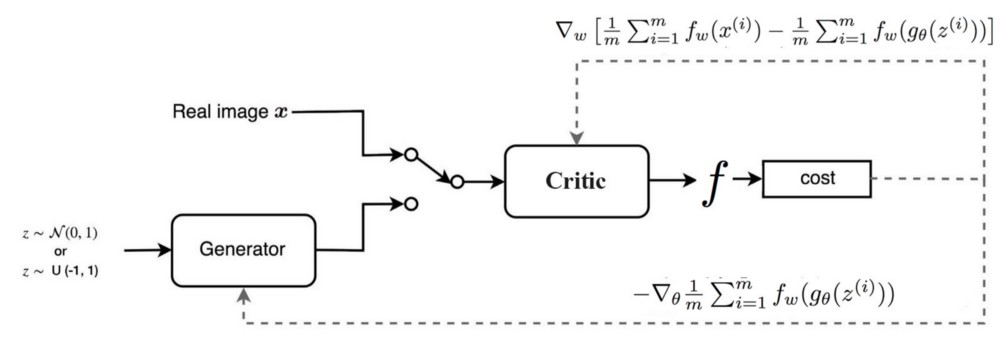
\includegraphics[scale=0.3]{wgan_training.jpeg}
    \caption{Architecture of a WGAN}
    \label{fig:cgan}
\end{figure}
\end{frame}

\begin{frame}
\frametitle{Conditional Generative Adversarial Network}
\begin{figure}[ht]
    \includegraphics[scale=0.285]{conditional_gan.png}
    \caption{Comparison between a regular GAN and a CGAN}
    \label{fig:cgan}
\end{figure}
\end{frame}

\begin{frame}
\frametitle{Feature extraction via Transfer learning}
\begin{itemize}
\item Transfer learning - using a neural network trained at solving one problem to solve different, but similar problem
\item VGG16 - convolutional neural network trained at classifying objects from the famous dataset ImageNet
\end{itemize}

\begin{figure}[ht]
    \centering
    \includegraphics[scale=0.225]{vgg16.png}
    \caption{Architecture of VGG16 - deep convolutional neural network with 16 layers}
    \label{fig:vgg16}
\end{figure}

\end{frame}

\begin{frame}
\frametitle{Feature extraction via autoencoder}
\begin{figure}[ht]
    \centering
    \includegraphics[scale=0.12]{autoencoder.png}
    \caption{Architecture of an autoencoder}
    \label{fig:ae}
\end{figure}
\begin{equation}
    \phi:X \rightarrow F
\end{equation}
\begin{equation}
    \psi:F \rightarrow X
\end{equation}
\begin{equation}
\phi,\psi = \operatorname*{arg\,min}_{\phi,\psi} {\parallel}X - (\psi\circ\phi)X{\parallel}^2
\end{equation}
\end{frame}

\begin{frame}
\frametitle{K-means Clustering}
By using K-means clustering, we can group the images and create synthetic labels. Images that have more in common that they do with the other images will have the same label.
\begin{figure}[ht]
    \centering
    \includegraphics[scale=0.25]{kmeans.png}
    \caption{K-means clustering example}
    \label{fig:kmeans}
\end{figure}
\end{frame}

\begin{frame}
\frametitle{Image Processing Algorithms}
\begin{columns}
\column{0.3\textwidth}
\begin{itemize}
\item Blurring
\item Complementing
\item Color changing
\item Denoising Autoencoder
\end{itemize}
\column{0.5\textwidth}
\begin{figure}[ht]
    \includegraphics[scale=0.11]{denoising_autoencoder.png}
    \caption{Architecture of a Denoising Autoencoder}
    \label{fig:denoising_autoencoder}
\end{figure}
\end{columns}
\end{frame}

\begin{frame}
\frametitle{Implementation}
\begin{columns}
\column{0.3\textwidth}
\begin{itemize}
\item Python 3
\item Tensorflow 2.0
\item NumPy
\item OpenCV
\item Matplotlib
\item Scikit-learn
\item PIL
\item Django
\item HTML
\item CSS
\item JavaScript
\item Nvidia CUDA
\end{itemize}
\column{0.7\textwidth}
\begin{figure}[ht]
    \includegraphics[scale=0.12]{technologies.png}
    \label{fig:python}
\end{figure}
\end{columns}
\end{frame}

\begin{frame}
\frametitle{Results}
\begin{figure}[ht]
    \includegraphics[scale=0.55]{results.png}
    \caption{Sample of generated images}
    \label{fig:results}
\end{figure}
\end{frame}

\begin{frame}
\frametitle{Conclusion \& Future Work}
{\bf Conclusion:}
\bigbreak
\begin{itemize}
\item Pleasurable results, although graphic designers still cannot be completely replaced
\item Room for further improvements
\end{itemize}
\bigbreak
{\bf Future plans:}
\begin{itemize}
\item Train the neural networks for more iterations
\item Implement new image processing algorithms
\item Expand the research into other UI elements such as pictograms
\end{itemize}
\end{frame}

\begin{frame}
\frametitle{Personal contribution}
\begin{itemize}
\item Architecture + hyperparameter tuning
\item Development of a system, capable of producing great results
\item Clarification and addressing of the main challenges in UI elements synthesis
\end{itemize}
\end{frame}

\begin{frame}
	\frametitle{Demo}
	\centering{\url{https://calliope.pythonanywhere.com}}
\end{frame}


\begin{frame}
\centerline{\Huge Thank you for your attention!}
\centerline{\huge Any questions?}
\end{frame}

\end{document}
